\chapter{實驗結果與分析}
\label{cha:Evaluation}

此章節中,我們將針對前述第~\ref{cha:Method}~章之研究方法進行實驗結果評估與分析,第~\ref{sec:SystemStructure}~小節說明實驗系統架構、第~\ref{sec:DataPreprocessEvaluation}~小節說明資料前處理評估、第~\ref{sec:DataAnalysisEvaluation}~小節說明資料分析評估、第~\ref{sec:MachineLearningEvaluation}~小節說明機器學習評估、第~\ref{sec:PredictionResultAnalysisEvaluation}~小節說明預測結果分析評估,以及第~\ref{sec:ApplicationAnalysisEvaluation}~小節說明產業應用分析評估。

\section{實驗系統架構}
\label{sec:SystemStructure}

本論文實驗系統架構將分為資料前處理端、資料分析端與機器學習端,如~\ref{tab:ResearchEnvironment},並均以 Python 3.9.7 做為開發語言。

\begin{itemize}
    \item [■] 資料前處理端:以 Apache Spark 3.2.1~\cite{armbrust2015spark}處理資料之前處理以及分割資料集所使用。
    \item [■] 資料分析端:以 missingno 0.5.1~\cite{Bilogur2018}、Seaborn 0.11.2~\cite{michael_waskom_2020_3767070}協助以圖表方式呈現資料特性。
    \item [■] 機器學習端:以 pandas 1.3.4~\cite{jeff_reback_2020_3715232}~\cite{mckinney-proc-scipy-2010}、scikit-learn 0.24.2~\cite{scikit-learn}~\cite{sklearn_api}、XGBoost 1.6.1~\cite{chen2016xgboost}處理機器學習訓練與評估。
\end{itemize}

\begin{table}[!htb]
	\centering
	\begin{tabular}{cclclcl}
	\hline \hline
	系統端點 && 資料前處理端 && 資料分析端 && 機器學習端 \\
    \hline \hline
    \multirow{3}*{研究環境} && \emph{Apache Spark} && \emph{missingno} && \emph{pandas} \\
    &&&& \emph{Seaborn} && \emph{scikit-learn} \\
    &&&&&& \emph{XGBoost} \\
    \hline \hline
	\end{tabular}
	\caption[實驗系統架構之研究環境表]{實驗系統架構之研究環境表}
	\label{tab:ResearchEnvironment}
\end{table}

本文的資料集取自一博弈遊戲,此遊戲於全球發行,遊戲內容包含了老虎機 ( Fruit Machine )、魚機 ( Fish Hunter ) 和其他小遊戲。
\newpage

\section{資料前處理評估}
\label{sec:DataPreprocessEvaluation}

此階段將評估前章~\ref{sec:DataPreProcess} 小節之資料前處理。~\ref{subsec:AudienceEvaluation} 小節為預測受眾評估,將說明~\ref{subsec:DataFilter} 小節之資料過濾;~\ref{subsec:FeatureEvaluation} 小節為預測特徵評估,將說明~\ref{subsec:ClassPreparation} 小節之目標值準備及~\ref{subsec:FeatureMining} 小節之資料特徵探勘與特徵工程。

本文收集了 2022/03/01 至 2022/05/31 的資料,共計三個月。此資料集是以天為單位,記錄了玩家於遊戲平台上和各項遊戲內的行為軌跡。總容量約為 44 GB。

\subsection{預測受眾評估}
\label{subsec:AudienceEvaluation}

本文將日本新進玩家作為預測受眾,因為日本玩家相較於其他國家較少有不良的帳號紀錄\ (\ 例如:同一位玩家多次創建新帳號等\ ),其遊戲資料相對地會較有可信度。此外,本文特別排除了等級 10 以下的玩家,確保收集到的玩家資料皆是有通過新手教學的,讓後續產生的特徵更有價值。共有 60,469 位玩家作為預測受眾,來進行後續實驗。

接著進行資料過濾,以獲得有價值玩家。本文直接鎖定預測受眾於日本等級10以上之新進玩家,用到的資料集沒有空缺值存在,因此,會直接進行無價值玩家資料處理。本文根據市場操作人員的建議,將觀察期 ( $O$ )、挽留期 ( $R$ ) 及表現期 ( $P$ ) 分別設為 4 天、1 天及 2 天,將無價值玩家排除後,最後剩下 57,170 位有價值玩家,如表~\ref{tab:ValuePlayerObservation}。

\begin{table}[!htb]
	\centering
	\begin{tabular}{ccccc}
	\hline \hline
	新進玩家總數 & \tabincell{c}{日本等級10以上\\新進玩家數} & 空缺值玩家數 & 無價值玩家數 & 有價值玩家數 \\
    \hline \hline
    4,750,383 & 60,469 & 0 & 3,299 & 57,170 \\
    \hline
    \multicolumn{5}{c}{有價值玩家數 $=$ 日本等級10以上新進玩家數 $-$ 空缺值玩家數 $-$ 無價值玩家數} \\
    \hline \hline
	\end{tabular}
	\caption[有價值玩家觀察表]{有價值玩家觀察表}
	\label{tab:ValuePlayerObservation}
\end{table}
\newpage

\subsection{預測特徵評估}
\label{subsec:FeatureEvaluation}

圖~\ref{fig:eva_PlayerChurnPeriod} 為新進玩家之流失長條圖,用來觀察有價值玩家的流失速度。從圖中可以看出,隨著天數增加,有登入遊戲之玩家數量會跟著減少,創帳號後隔天有登入紀錄的玩家有 6 成左右,創帳號後第 3 天有登入紀錄者只剩下不到 4 成。故本論文聚焦於新進玩家之流失預測,希望能快速進行挽留策略,把握住新進玩家。

\begin{figure}[!htb]
    \begin{center}
      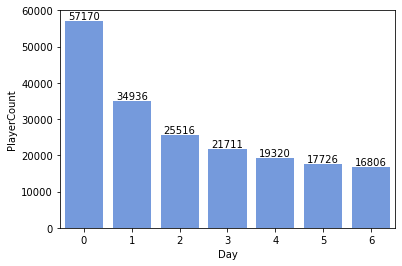
\includegraphics[width=0.7\textwidth]{figures/evaluation/Image_PlayerChurnPeriod.png}
      \caption[新進玩家之流失長條圖]{新進玩家之流失長條圖(x 軸為玩家登入日減去創立帳號日;y 軸為有登入之玩家數)}
      \label{fig:eva_PlayerChurnPeriod}
    \end{center}
\end{figure}

本文將定義新進玩家\ (\ 於~\ref{subsec:AudienceEvaluation}~小節中,篩選後之有價值玩家\ )\ 中的非流失玩家與流失玩家。觀察期有登入紀錄的玩家中,表現期間也有登入紀錄者視為非流失玩家,反之視為流失玩家。如表~\ref{tab:ChurnPlayerAndNonChurnPlayerDefinition},會有 20,488 位非流失玩家及 36,682 位流失玩家來做後續實驗。

\begin{table}[!htb]
	\centering
	\begin{tabular}{ccccc}
	\hline \hline
	有價值玩家數 & 非流失玩家 & 非流失玩家占比 & 流失玩家數 & 流失玩家占比 \\
    \hline \hline
    57,170 & 20,488 & 35.84 \% & 36,682 & 64.16 \% \\
    \hline \hline
	\end{tabular}
	\caption[非流失玩家及流失玩家定義表]{非流失玩家及流失玩家定義表}
	\label{tab:ChurnPlayerAndNonChurnPlayerDefinition}
\end{table}
\newpage

從原始資料集中探勘出$O$天\ (\ 資料特徵探勘期,即觀察期\ )\ 內之玩家資料,並以此來建立資料特徵。以計次、加總與平均,並以天為單位拆分時間段,產生第一層特徵變數,再對第一層特徵變數做計算,進而得到第二層特徵變數。最後,第一層特徵有156個,第二層特徵有93個,共得到了 249 個特徵變數。

另外,因類別型資料特徵不適用於樹狀結構之學習模型,故在其應用於機器學習前,將此類資料特徵透過 One Hot Encoding~\cite{wiki:OneHotEncoding}進行轉化,以利機器學習訓練,將此類特徵也歸類至第一層特徵,如圖~\ref{fig:eva_OneHotEncoder} 之作業系統。因此,第一層特徵數為 158 個,總特徵數為 251 個。

\begin{figure}[!htb]
    \begin{center}
      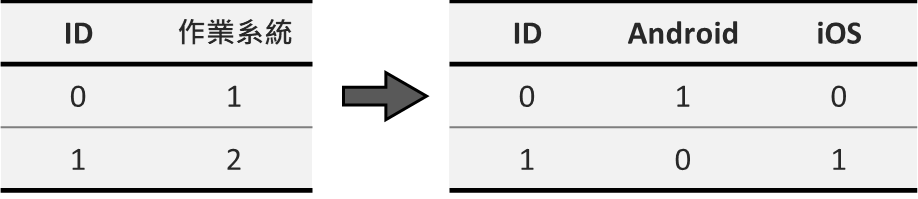
\includegraphics[width=0.75\textwidth]{figures/evaluation/Image_OneHotEncoder.png}
      \caption[作業系統 One Hot Encoding]{作業系統 One Hot Encoding (作業系統1為Android;2為iOS)}
      \label{fig:eva_OneHotEncoder}
    \end{center}
\end{figure}

為了避免特徵之間存在高度相關性,會影響到模型預測的準確性,本文對上述 251 個特徵變數進行篩選。透過支持向量機 ( Support Vector Machine ) 找出高共線性的冗贅特徵,並將其排除,最後只剩下 52 個特徵變數。此外,去掉高共線性的特徵也可以讓模型的可解釋性更好。表~\ref{tab:NumberOfFeatures} 為資料特徵總數表。圖~\ref{fig:eva_FirstFeatures} 為第一層變數圖、圖~\ref{fig:eva_SecondFeatures} 為第二層變數圖,而紅色底為篩選後之特徵。

\begin{table}[!htb]
	\centering
	\begin{tabular}{cccc}
	\hline \hline
	第一層特徵數 & 第二層特徵數 & 篩選前特徵數 & 篩選後特徵數 \\
    \hline \hline
    158 & 93 & 251 & 52 \\
    \hline \hline
	\end{tabular}
	\caption[資料特徵總數表]{資料特徵總數表}
	\label{tab:NumberOfFeatures}
\end{table}

為了避免部分特徵之數值過大或過小,彼此間差距較大,會影響到模型訓練精度,本文對所有特徵數值進行歸一化 ( Normalization )。式~\ref{eq:Normalization} 為本文歸一化的方式,會將所有數值映射到 [0,1] 區間。

\begin{equation}
  \label{eq:Normalization}
  x' = \frac{x-min(x)}{max(x)-min(x)}
\end{equation}
\newpage

\begin{figure}[!htb]
    \begin{center}
      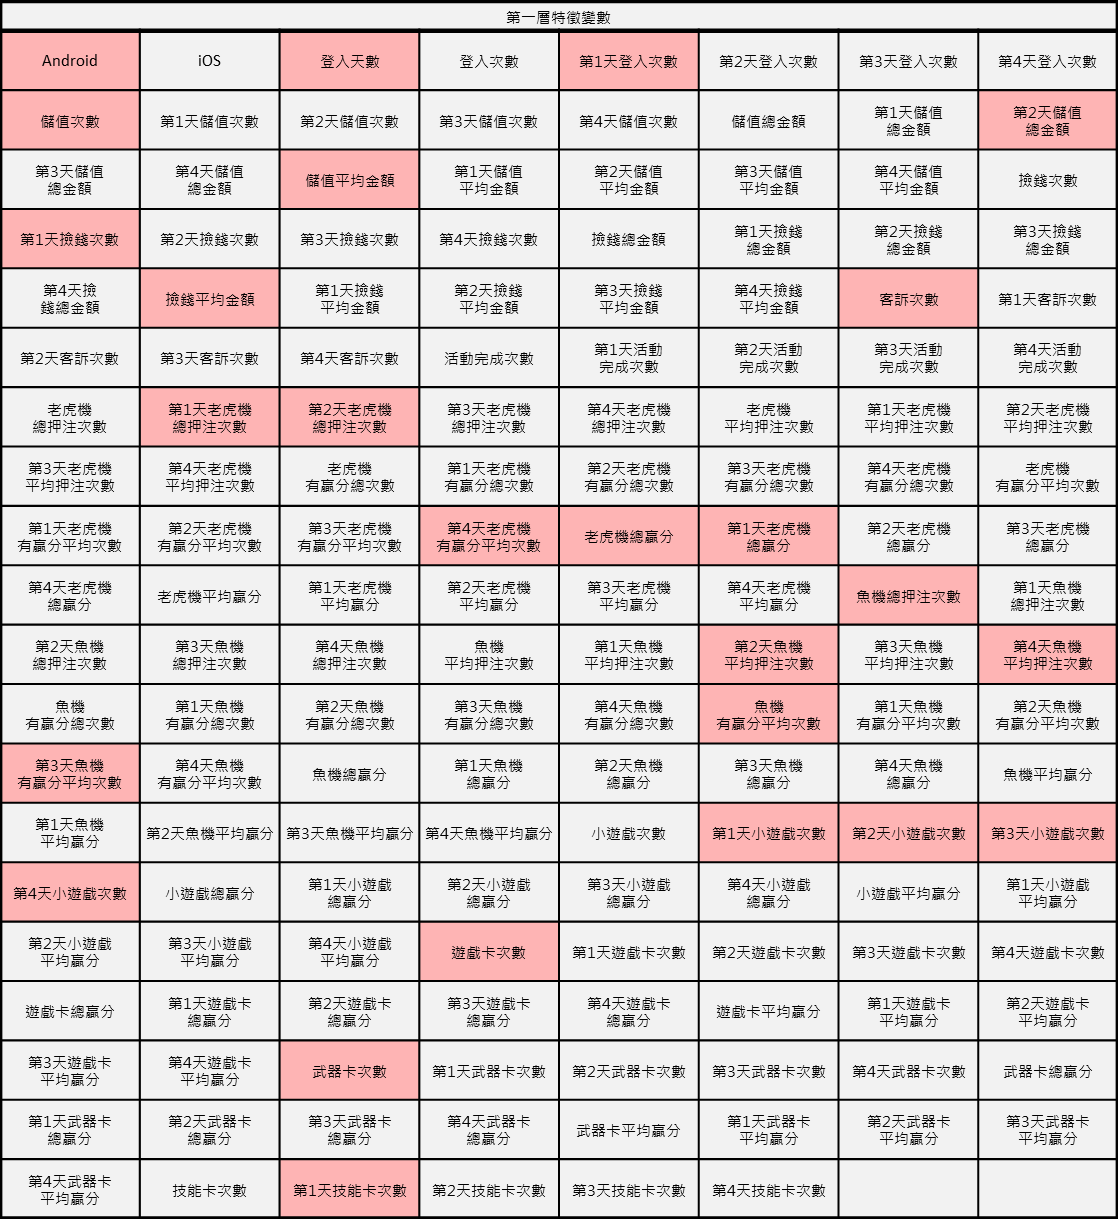
\includegraphics[width=1\textwidth]{figures/evaluation/Image_FirstFeatures.png}
      \caption[第一層特徵變數]{第一層特徵變數\ (\ 紅色底為篩選後之特徵\ )}
      \label{fig:eva_FirstFeatures}
    \end{center}
\end{figure}

\begin{figure}[!htb]
    \begin{center}
      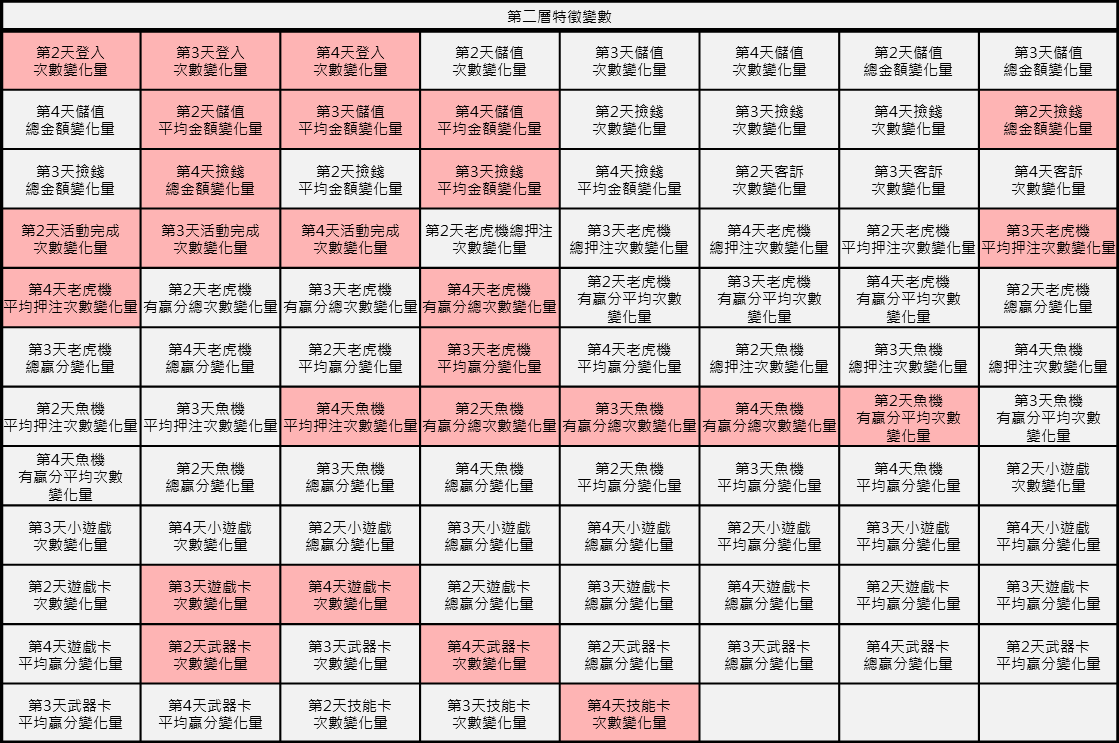
\includegraphics[width=1\textwidth]{figures/evaluation/Image_SecondFeatures.png}
      \caption[第二層特徵變數]{第二層特徵變數\ (\ 紅色底為篩選後之特徵\ )}
      \label{fig:eva_SecondFeatures}
    \end{center}
\end{figure}
\newpage

\section{資料分析評估}
\label{sec:DataAnalysisEvaluation}

此階段將評估前章 \ref{subsubsec:ValuableFeatures}~小節之高資訊量資料特徵推測,於 \ref{subsec:EDAEvaluation}~小節\ 探索性資料分析評估說明。

\subsection{探索性資料分析評估}
\label{subsec:EDAEvaluation}

利用長條圖及直方圖觀察在資料集中哪些特徵可能屬於高資訊量資料特徵。

圖~\ref{fig:eva_ValuableFeature_LoginDays} 為觀察期間玩家登入天數之人數統計圖。可以從圖中看出,非流失玩家數會隨著登入天數增加而遞增,流失玩家數則隨著登入天數增加而遞減。推測玩家登入天數可以帶給學習模型很好的分類資訊。

\begin{figure}[!htb]
    \begin{center}
      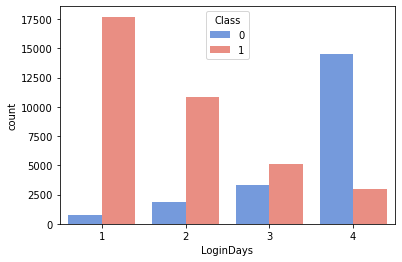
\includegraphics[width=0.7\textwidth]{figures/evaluation/Image_LoginDays.png}
      \caption[觀察期間玩家登入天數之人數統計圖]{觀察期間玩家登入天數之人數統計圖\ (\ x 軸為登入天數;y 軸為玩家數量\ )\ }
      \label{fig:eva_ValuableFeature_LoginDays}
    \end{center}
\end{figure}
\newpage

圖~\ref{fig:eva_ValuableFeature_DailyActivityMissionTimes} 為觀察期間玩家完成活動任務之次數統計圖。可以從圖中看出,除了創帳號當天以外,非流失玩家完成活動任務的次數皆遠大於流失玩家,甚至於創帳號後第三天,其次數變化量還為正值。推測活動任務完成次數之相關特徵可以帶給學習模型很好的分類資訊。

\begin{figure}[!htb]
    \begin{center}
      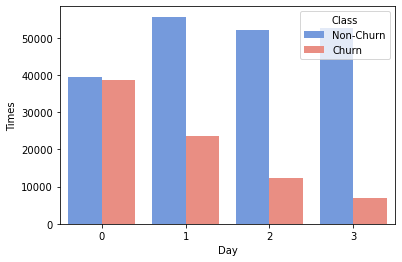
\includegraphics[width=0.7\textwidth]{figures/evaluation/Image_DailyActivityMissionTimes.png}
      \caption[觀察期間玩家完成任務之次數統計圖]{觀察期間玩家完成任務之次數統計圖\ (\ x 軸為觀察期第 x 天;y 軸為活動任務完成次數\ )\ }
      \label{fig:eva_ValuableFeature_DailyActivityMissionTimes}
    \end{center}
\end{figure}
\newpage

圖~\ref{fig:eva_ValuableFeature_D3SlotsMeanWinTimes} 為玩家創帳號後第三天之老虎機有贏分平均次數統計圖。可以從圖中看出,到了創帳號後第三天,流失玩家幾乎都沒有獲得贏分。推測此特徵可以帶給學習模型很好的分類資訊。

\begin{figure}[!htb]
    \begin{center}
      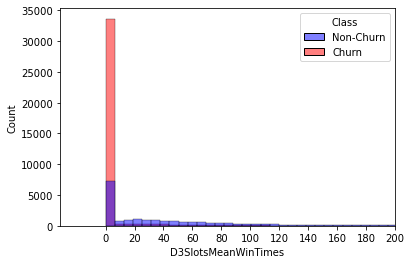
\includegraphics[width=0.7\textwidth]{figures/evaluation/Image_D3SlotsMeanWinTimes.png}
      \caption[玩家創帳號後第三天之老虎機有贏分平均次數統計圖]{玩家創帳號後第三天之老虎機有贏分平均次數\ (\ x 軸為平均有贏分次數;y 軸為玩家數量\ )\ (\ 紫色區域為非流失玩家與流失玩家重疊區域\ )\ }
      \label{fig:eva_ValuableFeature_D3SlotsMeanWinTimes}
    \end{center}
\end{figure}

圖~\ref{fig:eva_ValuableFeature_SystemType} 為作業系統各玩家統計圖。可以從圖中看出,不論是何種作業系統,流失玩家與非流失玩家的比例都差不多。推測作業系統的差異無法帶給學習模型很好的分類資訊。

\begin{figure}[!htb]
    \begin{center}
      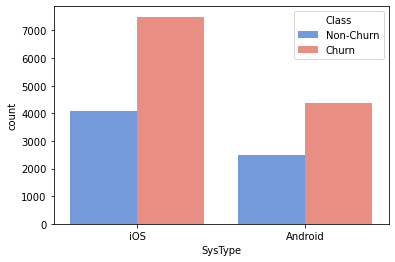
\includegraphics[width=0.7\textwidth]{figures/evaluation/Image_SystemType.png}
      \caption[作業系統各玩家統計圖]{作業系統各玩家統計圖\ (\ x 軸為作業系統;y 軸為玩家數量\ )\ }
      \label{fig:eva_ValuableFeature_SystemType}
    \end{center}
\end{figure}

\section{機器學習評估}
\label{sec:MachineLearningEvaluation}

此階段將評估前章~\ref{sec:MachineLearning} 小節之機器學習。~\ref{subsec:SplitDatasetEvaluation} 小節為分割訓練與測試資料集評估,將說明~\ref{subsec:SplitDataset} 小節之分割訓練與測試資料集;~\ref{subsec:ImbalancedDataHandleEvaluation} 小節為不平衡資料權重調整評估,將說明~\ref{subsec:ImbalancedDataHandle} 小節之不平衡資料權重調整;~\ref{subsec:BestModelEvaluation} 小節為最佳模型評估,將說明~\ref{subsec:TuningBestParams} 小節之搜尋最佳參數解及~\ref{subsec:EvaluateBestModel} 小節之評估驗證最佳模型;~\ref{subsec:TemporalWindowEvaluation} 小節為時間框架評估,將比較觀察期、表現期不同的天數,會對模型的輸出有甚麼影響。

\subsection{分割訓練與測試資料集評估}
\label{subsec:SplitDatasetEvaluation}

將資料集依照 8:2 之比例分割。如圖~\ref{fig:Image_SplitDataset},採分類隨機抽樣,即流失玩家與非流失玩家各別以 8:2 之比例隨機抽樣。表~\ref{tab:NumberOfSplitedPayerAndNonPayer} 為分割完資料集後之流失玩家數與非流失玩家數,訓練資料集與測試資料集之流失玩家與非流失玩家比例皆與原資料集相等,約為 1.79 倍。

\begin{table}[!htb]
	\centering
	\begin{tabular}{|c|r|r|}
	\hline \hline
	\diagbox{資料集}{玩家數} & 流失玩家 & 非流失玩家 \\
    \hline \hline
    訓練集 & 29,346 & 16,390 \\
    \hline
    測試集 & 7,336 & 4,098 \\
    \hline \hline
	\end{tabular}
	\caption[訓練與測試資料集玩家數表]{訓練與測試資料集玩家數表}
	\label{tab:NumberOfSplitedPayerAndNonPayer}
\end{table}

\subsection{資料不平衡處理評估}
\label{subsec:ImbalancedDataHandleEvaluation}

依照式~\ref{eq:SampleWeightFormula} 計算流失玩家樣本之縮小權重,如式~\ref{eq:SampleWeightCalculation},最後將流失玩家之樣本權重縮小 0.56 倍。

\begin{equation}
    \label{eq:SampleWeightCalculation}
    class\ 0 : class\ 1 = 1 : \frac{16,390}{29,346} = 1 : 0.56
\end{equation}
\newpage

圖~\ref{fig:eva_ROCCurveEvaluationImbalancedData} 為三種學習模型之ROC Curve,並比較不平衡資料處理前後之差異,(a)為決策樹、(b)為隨機森林、(c)為極限梯度提升,黃色線為未加入權重值、藍色線為加入權重值。從圖組中可以看出,在流失玩家之樣本權重上進行縮小,於本文並沒有明顯的作用,推測是因為本文預測的受眾資料並沒有極大的不平衡。

\begin{figure}[!htb]
    \centering
    \subfigure[決策樹ROC Curve圖] {
      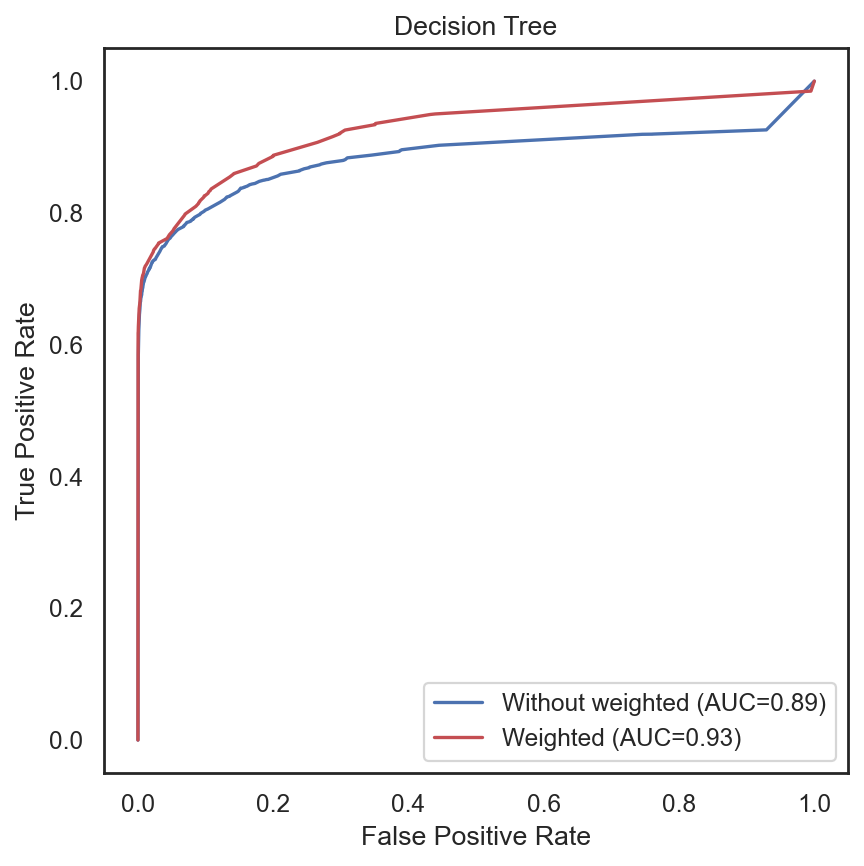
\includegraphics[width=0.47\columnwidth]{figures/evaluation/Image_DTROCCurve.png}
    }
    \subfigure[隨機森林ROC Curve圖] {
        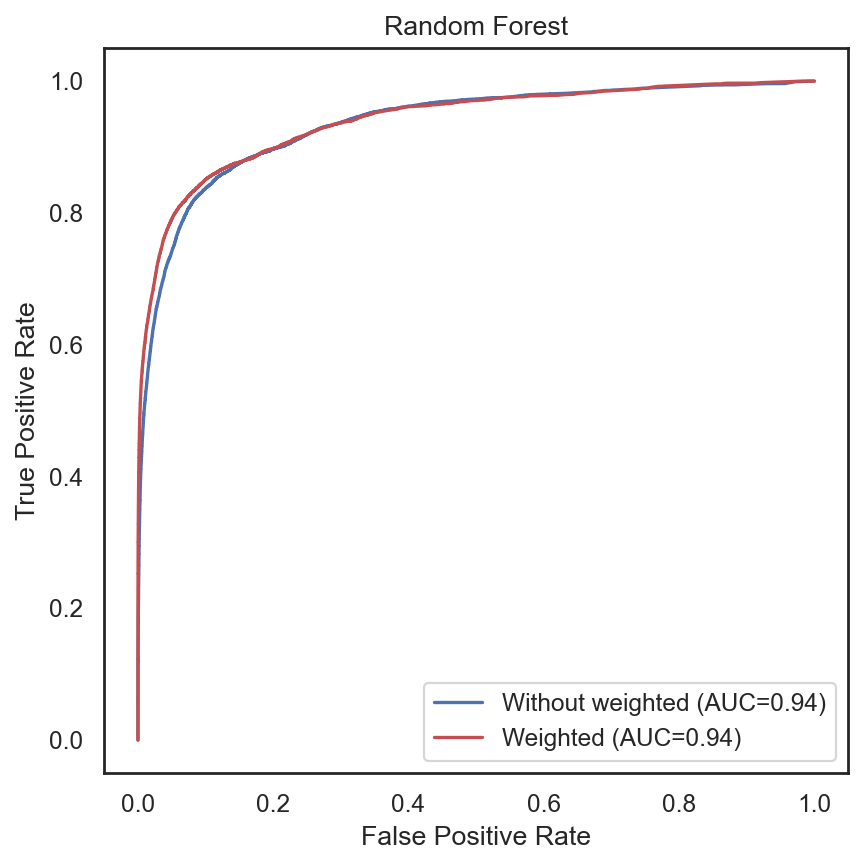
\includegraphics[width=0.47\columnwidth]{figures/evaluation/Image_RFROCCurve.png}
    }
    \subfigure[極限梯度提升ROC Curve圖] {
        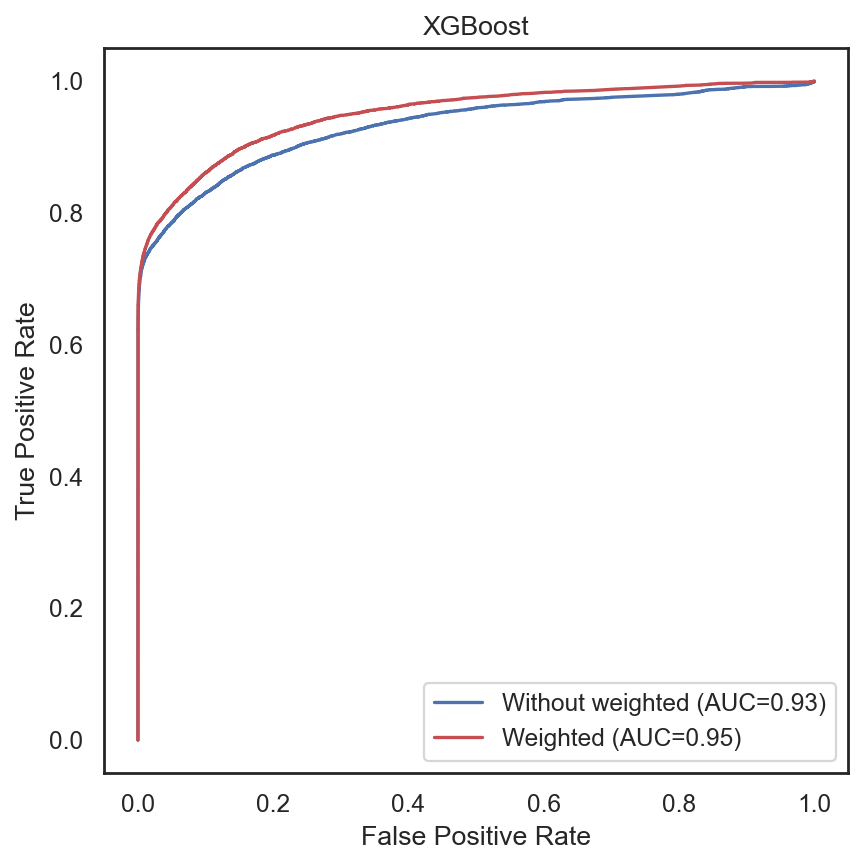
\includegraphics[width=0.47\columnwidth]{figures/evaluation/Image_XGBROCCurve.png}
    }
    \caption[不平衡資料處理前後比較之ROC Curve圖]{不平衡資料處理前後比較之ROC Curve圖\ (\ x 軸為假陽率;y 軸為真陽率\ )}
    \label{fig:eva_ROCCurveEvaluationImbalancedData}
\end{figure}
\newpage

圖~\ref{fig:eva_PRCurveEvaluationImbalancedData} 為三種學習模型之PR Curve,並比較不平衡資料處理前後之差異,(a)為決策樹、(b)為隨機森林、(c)為極限梯度提升,黃色線為未加入權重值、藍色線為加入權重值。從圖組中可以看出,在流失玩家之樣本權重上進行縮小,於本文並沒有明顯的作用,推測是因為本文預測的受眾資料並沒有極大的不平衡。

\begin{figure}[!htb]
    \centering
    \subfigure[決策樹PR Curve圖] {
      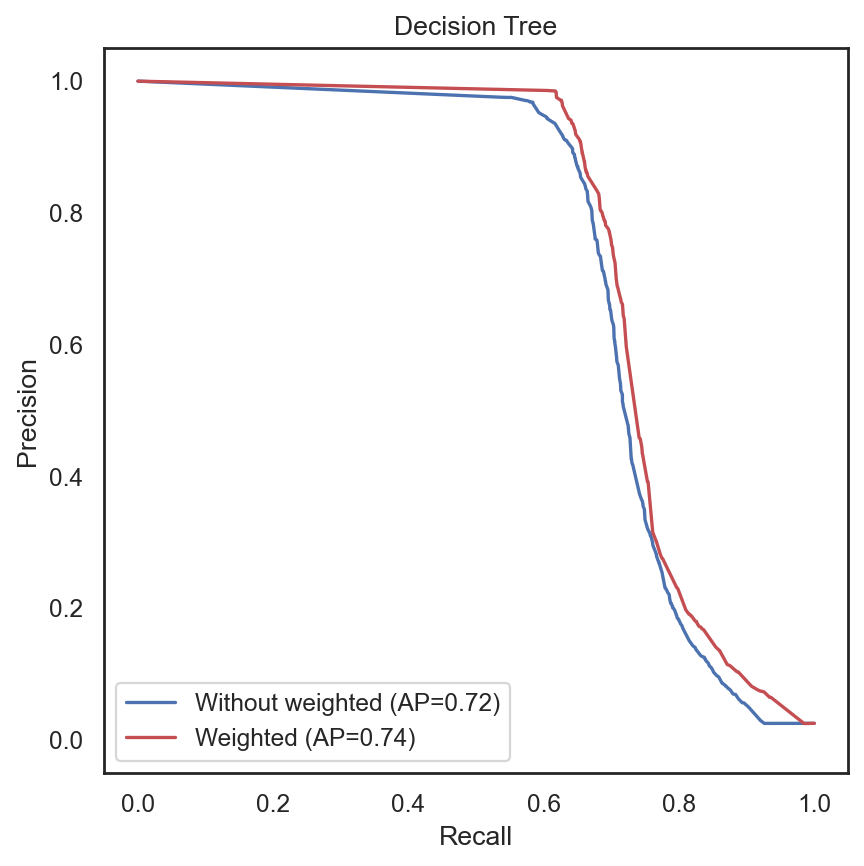
\includegraphics[width=0.47\columnwidth]{figures/evaluation/Image_DTPRCurve.png}
    }
    \subfigure[隨機森林PR Curve圖] {
        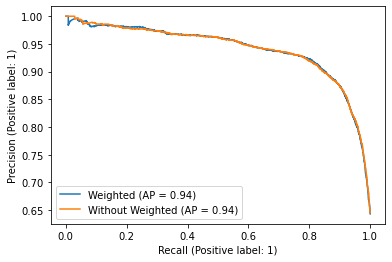
\includegraphics[width=0.47\columnwidth]{figures/evaluation/Image_RFPRCurve.png}
    }
    \subfigure[極限梯度提升PR Curve圖] {
        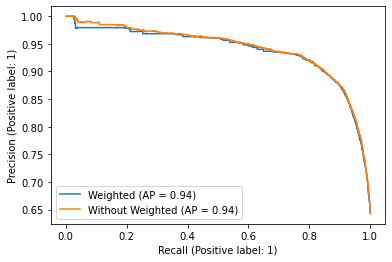
\includegraphics[width=0.47\columnwidth]{figures/evaluation/Image_XGBPRCurve.png}
    }
    \caption[不平衡資料處理前後比較之PR Curve圖]{不平衡資料處理前後比較之PR Curve圖\ (\ x 軸為召回率;y 軸為精確率\ )}
    \label{fig:eva_PRCurveEvaluationImbalancedData}
\end{figure}
\newpage

\subsection{最佳模型評估}
\label{subsec:BestModelEvaluation}

利用網格搜索與交叉驗證來調校出最佳模型。如圖~\ref{fig:Image_RepeatedStratifiedKFold},我們將採用Reapted 2次及5-Fold,最後使用測試資料集進行評估驗證,將說明 7,336 位流失玩家 ( $class\ 1$ ) 及 4,098 位非流失玩家 ( $class\ 0$ )。驗證結果如表~\ref{tab:BestModelEvaluation},從表中可以看出,極限梯度提升的結果表現為三種模型中最好的,因為其 Weighted F$_{\beta}$ - Score 為 0.849 是三者最高。

\begin{table}[!htb]
    \centering
        \begin{tabular}{|c|r|r|r|r|}
            \hline \hline
            \multirow{2}*{\diagbox{學習模型}{評估}} & $precision^+$ & $recall^+$ & ${F_{\beta}}^+$ & \multirow{2}*{$Weighted\ F_{\beta}$} \\
            \cline{2-4}
            & $precision^-$ & $recall^-$ & ${F_{\beta}}^-$ & \\
            \hline \hline
            \multirow{2}*{決策樹} & 0.892 & 0.863 & 0.870 & \multirow{2}*{0.846} \\
            \cline{2-4}
            & 0.769 & 0.813 & 0.802 & \\
            \hline
            \multirow{2}*{隨機森林} & 0.888 & 0.874 & 0.877 & \multirow{2}*{0.848} \\
            \cline{2-4}
            & 0.781 & 0.804 & 0.798 & \\
            \hline
            \multirow{2}*{極限梯度提升} & 0.887 & 0.876 & 0.878 & \multirow{2}*{0.849} \\
            \cline{2-4}
            & 0.783 & 0.801 & 0.796 & \\
            \hline
            \multicolumn{5}{|l|}{$+$:以正例(流失玩家 $class\ 1$ )為評估對象進行計算} \\
            \multicolumn{5}{|l|}{$-$:以反例(非流失玩家 $class\ 0$ )為評估對象進行計算} \\
            \hline \hline
        \end{tabular}
    \caption[最佳模型評估表]{最佳模型評估表}
    \label{tab:BestModelEvaluation}
\end{table}

圖~\ref{fig:eva_ModelsCurve} 為三種學習模型之曲線比較圖,(a) 為三種學習模型之ROC Curve比較圖、(b) 為三種學習模型之PR Curve比較圖,並且都為加入權重值之結果。從圖組中可以看出,隨機森林與極限梯度提升並沒有明顯的差異,原因可能在於特徵數量還不足夠,如果持續的擴增特徵,或許能凸顯出極限梯度提升的優點。

\begin{figure}[!htb]
    \centering
    \subfigure[三種學習模型之ROC Curve比較圖] {
      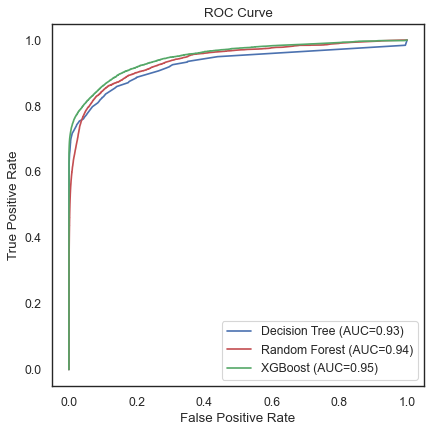
\includegraphics[width=0.48\columnwidth]{figures/evaluation/Image_ModelsROCCurve.png}
    }
    \subfigure[三種學習模型之PR Curve比較圖] {
        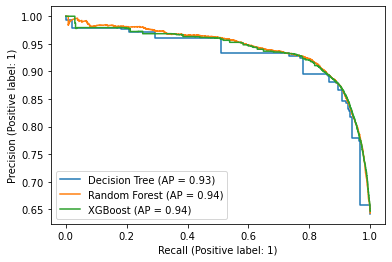
\includegraphics[width=0.48\columnwidth]{figures/evaluation/Image_ModelsPRCurve.png}
    }
    \caption[三種學習模型之曲線比較圖]{三種學習模型之曲線比較圖}
    \label{fig:eva_ModelsCurve}
\end{figure}

綜合上述得到的實驗結果,可以發現本文挑選的三種模型表現都不錯,Weighted F$_{\beta}$ - Score 都有接近 0.85,且曲線面積也都有 0.9 以上。可見本文建立的資料特徵能適用於各種模型中,並都有不錯的結果。

此外,極限梯度提升是採用梯度下降法 ( Gradient Descent ) 來加速學習模型之收斂,減少建樹時間成本,也較不會有過擬合 ( Overfitting ) 的情形出現。在訓練極限梯度提升模型時,可以將資料格式轉為極限梯度提升專用的 DMatrix 格式,以此來提升演算的效率。

表~\ref{tab:BestModelParams} 為三種學習模型之最佳參數解,參數搜尋範圍如表~\ref{tab:ParamsSearchRange}。決策樹因其為單樹結構,相較之下需要生成更深的樹;而隨機森林及極限梯度提升則因其為多樹結構,希望能以廣度發展,而非深度,相較之下需要生成更多的樹。

\begin{table}[!htb]
    \centering
        \begin{tabular}{clll}
            \hline \hline
            學習模型 & 決策樹 & 隨機森林 & 極限梯度提升 \\
            \hline \hline
            \multirow{4}*{參數調校} & max\char`_depth=5 & n\char`_estimators=60 & n\char`_estimators=25 \\
            & min\char`_samples\char`_split=2 & max\char`_depth=14 & max\char`_depth=5 \\
            & min\char`_samples\char`_leaf=20 & min\char`_samples\char`_split=6 & learning\char`_rate=0.05 \\
            && min\char`_samples\char`_leaf=5 & \\
            \hline \hline
        \end{tabular}
    \caption[最佳模型參數解表]{最佳模型參數解表}
    \label{tab:BestModelParams}
\end{table}

\begin{table}[!htb]
    \centering
        \begin{tabular}{cl}
            \hline \hline
            參數名 & 搜尋範圍 \\
            \hline \hline
            n\char`_estimators & 20, 25, 30, 35, 40, 45, 50, 55, 60 \\
            \hline
            max\char`_depth & 5, 6, 7, 8, 9, 10, 11, 12, 13, 14 \\
            \hline
            min\char`_samples\char`_split & 2, 4, 6, 8, 10 \\
            \hline
            min\char`_samples\char`_leaf & 1, 5, 10, 15, 20 \\
            \hline
            learning\char`_rate & 0.05, 0.07, 0.08, 0.1, 0.2 \\
            \hline \hline
        \end{tabular}
    \caption[參數搜尋範圍表]{參數搜尋範圍表}
    \label{tab:ParamsSearchRange}
\end{table}

\subsection{時間框架評估}
\label{subsec:TemporalWindowEvaluation}

將比較觀察期與表現期在不同天數的情況下,會對模型的輸出結果有甚麼影響,並用極限梯度提升來進行驗證。
\newpage

表~\ref{tab:BestObservationEvaluation} 為觀察期評估表,將挽留期及表現期設為1天及2天,並比較觀察期為2天、4天與6天的模型驗證結果。從表中可以看出,當觀察期越長時,模型的 Weighted F$_{\beta}$ - Score 越高,表示模型的表現結果越好。推測原因在於本文建立特徵的方式,因為能拆分更多的時間段,以此來獲得更多的玩家資料與特徵。

\begin{table}[!htb]
    \centering
        \begin{tabular}{|c|r|r|r|r|r|}
            \hline \hline
            \multirow{2}*{\diagbox{觀察期}{評估}} & $sample^+$ & $precision^+$ & $recall^+$ & ${F_{\beta}}^+$ & \multirow{2}*{$Weighted\ F_{\beta}$} \\
            \cline{2-5}
            & $sample^-$ & $precision^-$ & $recall^-$ & ${F_{\beta}}^-$ & \\
            \hline \hline
            \multirow{2}*{2天} & 6,570 & 0.834 & 0.767 & 0.790 & \multirow{2}*{0.780} \\
            \cline{2-5}
            & 4,905 & 0.718 & 0.796 & 0.766 & \\
            \hline
            \multirow{2}*{4天} & 7,336 & 0.887 & 0.876 & 0.878 & \multirow{2}*{0.849} \\
            \cline{2-5}
            & 4,098 & 0.783 & 0.801 & 0.796 & \\
            \hline
            \multirow{2}*{6天} & 7,701 & 0.913 & 0.907 & 0.908 & \multirow{2}*{0.878} \\
            \cline{2-5}
            & 3,589 & 0.803 & 0.815 & 0.813 & \\
            \hline
            \multicolumn{6}{|l|}{$+$:以正例(流失玩家 $class\ 1$ )為評估對象進行計算} \\
            \multicolumn{6}{|l|}{$-$:以反例(非流失玩家 $class\ 0$ )為評估對象進行計算} \\
            \hline \hline
        \end{tabular}
    \caption[觀察期評估表]{觀察期評估表}
    \label{tab:BestObservationEvaluation}
\end{table}

表~\ref{tab:BestPerformanceEvaluation} 為表現期評估表,將觀察期及挽留期設為4天及1天,並比較表現期為2天、4天與6天的模型驗證結果。從表中可以看出,當表現期越長時,模型的 Weighted F$_{\beta}$ - Score 越低,表示模型的表現結果越差。推測原因在於,定義是否流失的時間太長,原本會被定義為流失玩家的人,可能會變成非流失玩家,導致模型的預測能力受到影響。

\begin{table}[!htb]
    \centering
        \begin{tabular}{|c|r|r|r|r|r|}
            \hline \hline
            \multirow{2}*{\diagbox{表現期}{評估}} & $sample^+$ & $precision^+$ & $recall^+$ & ${F_{\beta}}^+$ & \multirow{2}*{$Weighted\ F_{\beta}$} \\
            \cline{2-5}
            & $sample^-$ & $precision^-$ & $recall^-$ & ${F_{\beta}}^-$ & \\
            \hline \hline
            \multirow{2}*{2天} & 7,336 & 0.887 & 0.876 & 0.878 & \multirow{2}*{0.849} \\
            \cline{2-5}
            & 4,098 & 0.783 & 0.801 & 0.796 & \\
            \hline
            \multirow{2}*{4天} & 6,779 & 0.867 & 0.845 & 0.852 & \multirow{2}*{0.828} \\
            \cline{2-5}
            & 4,449 & 0.773 & 0.802 & 0.793 & \\
            \hline
            \multirow{2}*{6天} & 6,463 & 0.849 & 0.846 & 0.847 & \multirow{2}*{0.821} \\
            \cline{2-5}
            & 4,548 & 0.782 & 0.786 & 0.785 & \\
            \hline
            \multicolumn{6}{|l|}{$+$:以正例(流失玩家 $class\ 1$ )為評估對象進行計算} \\
            \multicolumn{6}{|l|}{$-$:以反例(非流失玩家 $class\ 0$ )為評估對象進行計算} \\
            \hline \hline
        \end{tabular}
    \caption[表現期評估表]{表現期評估表}
    \label{tab:BestPerformanceEvaluation}
\end{table}
\newpage

從上述兩個表格中可以發現,當觀察期越長時,模型表現會越好,因為得到的特徵變多了;而當表現期越長時,模型表現會越差,因為原本該被定義為流失玩家的人,可能被定義成非流失玩家。但最後還是要根據市場需求來定義時間框架。

\section{預測結果分析評估}
\label{sec:PredictionResultAnalysisEvaluation}

此階段將評估前章~\ref{sec:PredictionResultAnalysis} 小節之預測結果分析。~\ref{subsec:FeatureImportanceEvaluation} 小節為資料特徵重要性評估,將說明~\ref{subsec:FeatureImportanceAnalysis} 小節之資料特徵重要性分析。

\subsection{資料特徵重要性評估}
\label{subsec:FeatureImportanceEvaluation}

將利用式~\ref{eq:GiniImportanceFormula}、式~\ref{eq:SingleTreeFeatureImportanceFormula} 及式~\ref{eq:ModelFeatureImportanceFormula} 計算之各資料特徵於各模型之資料特徵重要性。如圖~\ref{fig:eva_DTFeatureImportances}、圖~\ref{fig:eva_RFFeatureImportances} 及圖~\ref{fig:eva_XGBFeatureImportances},分別為決策樹、隨機森林及極限梯度提升之資料特徵重要性比較圖。

\begin{figure}[!htb]
    \begin{center}
      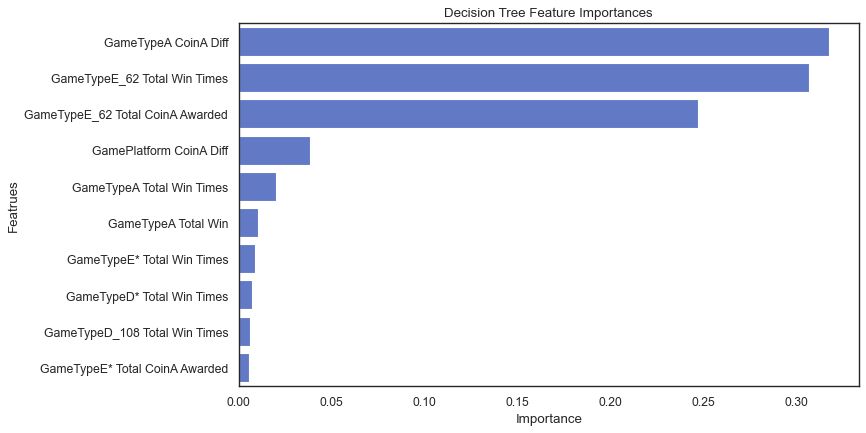
\includegraphics[width=1\textwidth]{figures/evaluation/Image_DTFeatureImportances.png}
      \caption[決策樹資料特徵重要性比較圖]{決策樹資料特徵重要性比較圖}
      \label{fig:eva_DTFeatureImportances}
    \end{center}
\end{figure}
\newpage

\begin{figure}[!htb]
    \begin{center}
      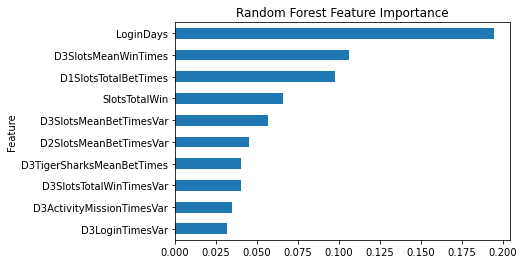
\includegraphics[width=1\textwidth]{figures/evaluation/Image_RFFeatureImportances.png}
      \caption[隨機森林資料特徵重要性比較圖]{隨機森林資料特徵重要性比較圖}
      \label{fig:eva_RFFeatureImportances}
    \end{center}
\end{figure}

\begin{figure}[!htb]
    \begin{center}
      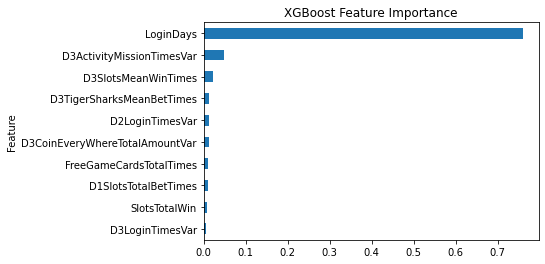
\includegraphics[width=1\textwidth]{figures/evaluation/Image_XGBFeatureImportances.png}
      \caption[極限梯度提升資料特徵重要性比較圖]{極限梯度提升資料特徵重要性比較圖}
      \label{fig:eva_XGBFeatureImportances}
    \end{center}
\end{figure}
\newpage

從三圖中可以看出,觀察期間的登入天數 ( LoginDays ) 皆是三種學習模型的第一名,可以說明登入天數的多寡確實與玩家是否流失有極大的關係。整合來看,在前十名中可以看到許多與變化量相關的特徵,如表~\ref{tab:FeatureImportanceTop10},雖不是主要原因,但可以從老虎機相關變化量特徵中說明,玩家是否流失確實與遊玩遊戲時的體驗起伏有關係。

\begin{table}[!htb]
    \centering
        \begin{tabular}{cl}
            \hline \hline
            參數名 & 代表意思 \\
            \hline \hline
            D2LoginTimesVar & 創帳號後第2天 登入次數變化量 \\
            \hline
            D3LoginTimesVar & 創帳號後第3天 登入次數變化量 \\
            \hline
            D2SlotsMeanWinVar & 創帳號後第2天 老虎機平均贏分變化量 \\
            \hline
            D2SlotsMeanBetTimesVar & 創帳號後第2天 老虎機平均押注次數變化量 \\
            \hline
            D3SlotsMeanBetTimesVar & 創帳號後第3天 老虎機平均押注次數變化量 \\
            \hline
            D3SlotsTotalWinTimesVar & 創帳號後第3天 老虎機有贏分總次數變化量 \\
            \hline
            D3ActivityMissionTimesVar & 創帳號後第3天 活動任務完成次數變化量 \\
            \hline
            D3CoinEveryWhereTotalAmountVar & 創帳號後第3天 撿錢總金額變化量 \\
            \hline \hline
        \end{tabular}
    \caption[特徵重要性前十名]{特徵重要性前十名\ (\ 變化量相關特徵\ )}
    \label{tab:FeatureImportanceTop10}
\end{table}

另外,三種學習模型之前十名資料特徵皆為數值型的資料特徵,而無類別型資料特徵,因其資料特徵重要性之評估以計算基尼重要性為主,數值型將會比類別型來得更為顯著,未來將可在計算重要性分析中,對於不同類型的資料特徵加入權重值,使得類別型的資料特徵能夠突出,讓整體分析更加準確。

\section{產業應用分析評估}
\label{sec:ApplicationAnalysisEvaluation}

此階段將評估前章~\ref{sec:ApplicationAnalysis} 小節之產業應用分析。~\ref{subsec:SurrogateModelEvaluation} 小節為代理人模型評估,將說明~\ref{subsec:SurrogateModel} 小節之代理人模型。

\subsection{代理人模型評估}
\label{subsec:SurrogateModelEvaluation}

代理人模型,以決策樹來說明極限梯度提升,能清楚地知道模型判斷是否流失的門檻,了解玩家流失的行為規則,在後續市場操作的策略上能有很好的建議。

圖~\ref{fig:eva_SurrogateModel} 為本文的代理人模型圖。從圖中來看,本文將數據集劃分為2個類別,即非流失玩家與流失玩家,其分別各占數據集的 0.36 與 0.64,所以最上面的根節點認為流失玩家的可能性較大。透過根節點可以知道,當玩家於觀察期間之登入天數\ (\ LoginDays\ )\ 小於 3 天時,有 69.4\% 的樣本數,且屬於流失玩家的可能性較大,因此會被判斷為流失玩家。繼續向下通過其他節點,分類結果就能更加確定。

此外,可以從代理人模型中發現,當登入天數小於 1 天時,流失機率已經高達 0.92。因此,可以建議遊戲商多推出留存規格,或是多舉辦與登入相關的活動,讓玩家增加其遊玩天數。

\begin{figure}[!htb]
    \begin{center}
      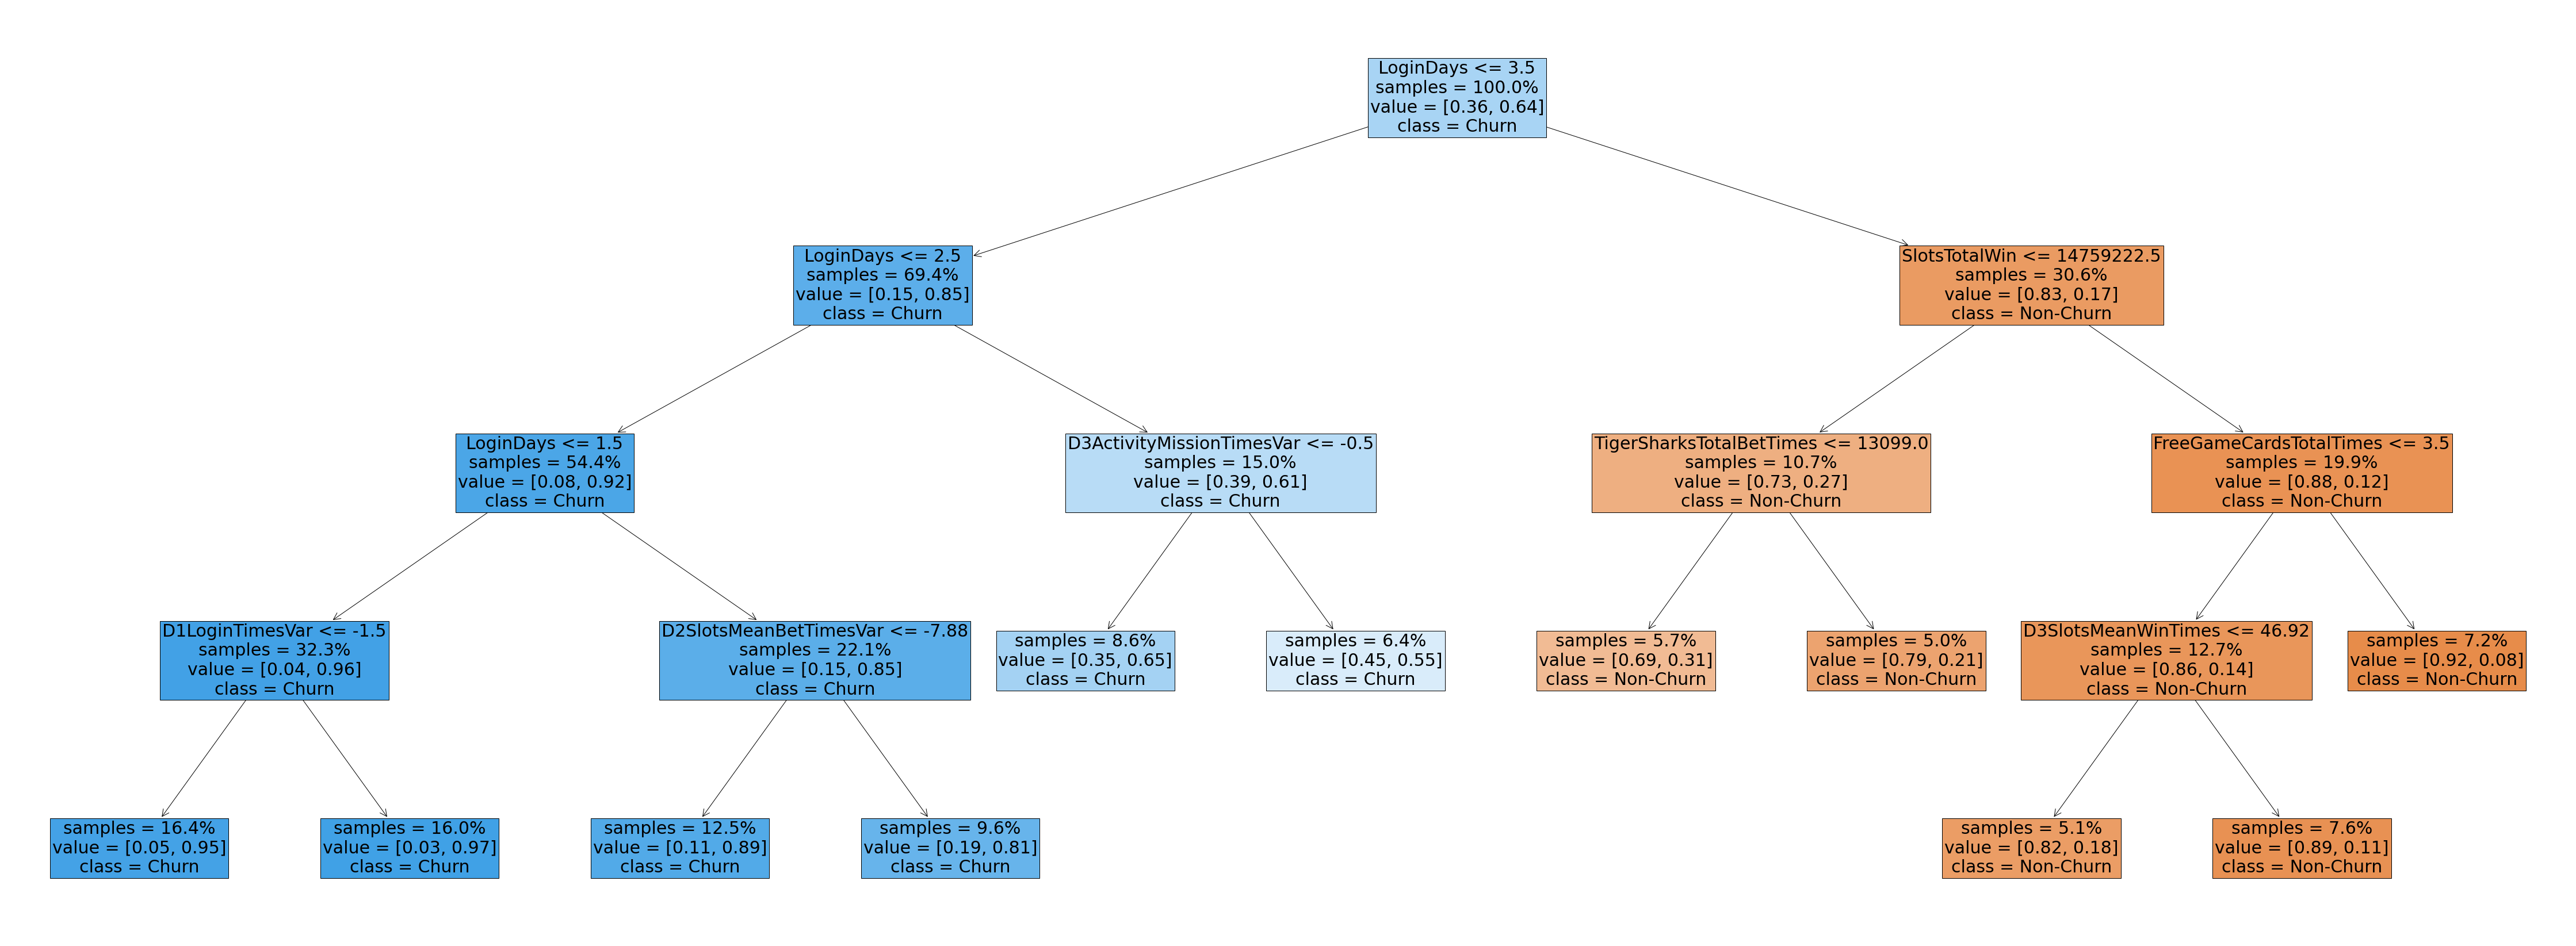
\includegraphics[width=1.5\textwidth, angle=90]{figures/evaluation/Image_SurrogateModel.png}
      \caption[代理人模型圖]{代理人模型圖}
      \label{fig:eva_SurrogateModel}
    \end{center}
\end{figure}
\newpage